%!TEX root = jir2018aspects.tex
\begin{table}
 \centering
    \caption{Behavioural and performance measures reported across the four experimental conditions (top table), systems and tasks (bottom table).}
    \label{tbl_actions}
    \renewcommand{\arraystretch}{1.4}
    %\begin{center}
    %\begin{small}
    \begin{tabulary}{\textwidth}{L{3.4cm}||D{1.55cm}|D{1.55cm}|D{1.55cm}|D{1.55cm}}
    %\begin{tabulary}{\textwidth}{|c||c|c|c|c|}
    \hline
    % OUTPUT FROM script
    & \multicolumn{4}{c}{\textbf{Experimental Conditions}} \\
    \cline{2-5}
    \textbf{Actions} & \textbf{\emph{D.As}} & \textbf{\emph{ND.As}} & \textbf{\emph{D.Ad}} & \textbf{\emph{ND.Ad}}\\  \hline\hline
    % START DATA
    \textbf{\emph{\#Queries}} & 5.92$\pm$ 0.88 & 5.25$\pm$ 0.80 & 4.96$\pm$ 0.74 & 5.20$\pm$ 0.69 \\ \hline
    \textbf{\emph{\#SERPs/Query}} & 1.78$\pm$ 0.14 & 2.42$\pm$ 0.24 & 2.28$\pm$ 0.31 & 2.28$\pm$ 0.20 \\ \hline
    \textbf{\emph{Documents/Query}} & 3.02$\pm$ 0.39 & 3.65$\pm$ 0.46 & 3.48$\pm$ 0.51 & 3.23$\pm$ 0.37 \\ \hline
    \textbf{\emph{Depth/Query}} & 12.85$\pm$ 1.49 & 15.73$\pm$ 1.45 & 16.19$\pm$ 2.14 & 13.94$\pm$ 1.93 \\ \hline\hline
    \textbf{\emph{\#Saved}} & 5.80$\pm$ 0.26 & 5.96$\pm$ 0.25 & 5.92$\pm$ 0.25 & 5.78$\pm$ 0.20 \\ \hline
    \textbf{\emph{\#TREC Saved}} & 2.63$\pm$ 0.22 & 2.18$\pm$ 0.23 & 2.51$\pm$ 0.23 & 2.22$\pm$ 0.22 \\ \hline
    \textbf{\emph{\#TREC Non-Relevant}} & 1.75$\pm$ 0.22 & 1.96$\pm$ 0.23 & 1.37$\pm$ 0.22 & 1.82$\pm$ 0.23  \\ \hline
    \textbf{\emph{\#Entities Found}} & 7.22$\pm$ 0.94* & 4.31$\pm$ 0.60* & 5.82$\pm$ 0.77 & 4.37$\pm$ 0.59*  \\ \hline
    \textbf{\emph{\#Docs w/ New Entities}} & 3.20$\pm$ 0.21* & 2.35$\pm$ 0.20* & 2.63$\pm$ 0.23 & 2.02$\pm$ 0.18* \\ \hline
    \end{tabulary}
    
    \vspace{5mm}
    
    \begin{tabulary}{\textwidth}{L{3.4cm}||D{1.55cm}|D{1.55cm}|D{1.55cm}|D{1.55cm}}
    %\begin{tabulary}{\textwidth}{|c||c|c|c|c|}
    \hline
         & \multicolumn{2}{c|}{\textbf{Systems}} & \multicolumn{2}{c}{\textbf{Tasks}} \\
         \cline{2-5}
 \textbf{Actions}       & \textbf{\emph{ND}} & \textbf{\emph{D}} & \textbf{\emph{Ad.}} & \textbf{\emph{As.}} \\
        \hline
        \hline
 \textbf{\emph{\#Queries}} & 5.23$\pm$ 0.53 & 5.44$\pm$ 0.58 & 5.08$\pm$ 0.51 & 5.59$\pm$ 0.59 \\ \hline
 \textbf{\emph{\#SERPs/Query}} & 2.35$\pm$ 0.16 & 2.03$\pm$ 0.17 & 2.28$\pm$ 0.18 & 2.10$\pm$ 0.14 \\ \hline
 \textbf{\emph{Documents/Query}} & 3.44$\pm$ 0.29 & 3.25$\pm$ 0.32 & 3.36$\pm$ 0.31 & 3.34$\pm$ 0.30 \\ \hline
 \textbf{\emph{Depth/Query}} & 14.84$\pm$ 1.58 & 14.52$\pm$ 1.31 & 15.07$\pm$ 1.44 & 14.29$\pm$ 1.47 \\ \hline\hline
 \textbf{\emph{\#Saved}} & 5.87$\pm$ 0.16 & 5.86$\pm$ 0.18 & 5.85$\pm$ 0.16 & 5.88$\pm$ 0.18 \\ \hline
 \textbf{\emph{\#TREC Saved}}  & 2.20$\pm$ 0.16 & 2.57$\pm$ 0.16 & 2.36$\pm$ 0.16 & 2.40$\pm$ 0.16 \\ \hline
    \textbf{\emph{\#TREC Non-Relevant}}  & 1.89$\pm$ 0.16 & 1.56$\pm$ 0.16 & 1.60$\pm$ 0.16 & 1.85$\pm$ 0.16 \\ \hline
    \textbf{\emph{\#Entities Found}}  & 4.34$\pm$ 0.42* & 6.52$\pm$ 0.61* & 5.10$\pm$ 0.49 & 5.76$\pm$ 0.57 \\ \hline
    \textbf{\emph{\#Docs w/ New Entities}} & 2.19$\pm$ 0.13* & 2.91$\pm$ 0.16* & 2.32$\pm$ 0.15* & 2.77$\pm$ 0.15* \\ \hline     

       % END DATA
    \end{tabulary}
    %\end{small}
    %\end{center}
\end{table}

%%%%%%%%%%%%%%%%%%%%%%%%%%%%%%%%%%%%%%%%%%%%%%%%%%%%%%%%%%%%%%%%%%%%%%%%%%%
\section{Results} \label{sec:results}
%%%%%%%%%%%%%%%%%%%%%%%%%%%%%%%%%%%%%%%%%%%%%%%%%%%%%%%%%%%%%%%%%%%%%%%%%%%

We now address our research questions and hypotheses as addressed in Section~\ref{sec:questions}. Both the behaviour and performance of each subject were analysed across each of the four experimental conditions, \textbf{\emph{D.As}}, \textbf{\emph{ND.As}}, \textbf{\emph{D.Ad}} and \textbf{\emph{ND.Ad}}. Task (\emph{\textbf{As}}. vs \emph{\textbf{Ad.}}) and system (\emph{\textbf{ND.}} vs \emph{\textbf{D.}}) effects were also examined. To evaluate these data, ANOVAs were conducted using the conditions, systems and tasks each as factors; main effects were examined with $\alpha=0.05$. Bonferroni tests were then used for post-hoc analysis. As discussed in Section~\ref{sec_measures}, $\alpha DCG$ values are computed using $\alpha=0.5$.

To begin our analysis, we first examined whether the performance experienced by participants on the two systems was, in fact, different (as indicated by our pilot study). We took the queries participants issued to each system and measured the performance according to $\alpha DCG$, aspectual recall and precision (see Table~\ref{tbl_queryperf_2018}). Statistical testing confirms that the two systems were significantly different in terms of diversity (i.e. $\alpha DCG@10$: $F(1, 1272)=28.74, p<0.001$, and $AR@10$: $F(1, 1272)=55.43, p<0.001$). $P@10$ was however not significantly different. This suggests that the reranking promoted relevant and diverse documents, but only in the top 10 results on average.
 
Aside from showing query performance, Table~\ref{tbl_queryperf_2018} also reports the number of terms issued per query over systems \textbf{\emph{ND}} and \textbf{\emph{D}}. Of the $1273$ queries issued, those issued to \textbf{\emph{ND}} were shorter on average, with $3.59$ terms compared to $3.80$ terms for \textbf{\emph{D}}. However, the vocabulary used by subjects issuing queries to \textbf{\emph{ND}} was more diverse than \textbf{\emph{D}} -- queries issued to \textbf{\emph{ND}} contained $345$ unique terms, compared to $292$ for \textbf{\emph{D}}.
This provides our first finding of note. When using \textbf{\emph{ND}}, participants issued more queries -- but were slightly shorter and more varied -- to accomplish their tasks. 

%%%%%%%%%%%%%%%
\subsection{Observed Behaviours}
%%%%%%%%%%%%%%%
\paragraph{Interactions.} Table~\ref{tbl_actions} presents the mean (and standard deviations) of: \textit{(i)} the number of queries issued; \textit{(ii)} the number of SERPs that were examined by subjects per query; \textit{(iii)} the number of documents examined (clicked) per query; and \textit{(iv)} the click depth (or search stopping depth) per query. %These mean values are compared in three ways: \emph{(i)} over each of the four experimental conditions trialled; \emph{(ii)} over the two experimental systems (non-diverse vs. diverse) and \emph{(iii)} over the two different search tasks (ad-hoc vs. aspectual). 
Statistical tests reveal no effects across conditions, systems or tasks. However, there are several trends that are worth mentioning. Firstly, we notice that when participants used the diversified system to complete the aspectual retrieval task, they examined fewer documents per query than when completing the same task on the non-diversified system (12.85 vs. 15.73) -- which is in line with \emph{\textbf{H1}}. We also observed that participants issued slightly more queries on the diversified system compared to the non-diversified system with the aspectual retrieval task (5.92 vs. 5.25) -- which is in line with \emph{\textbf{H2a}}. To reiterate however, these results were not significant.

%Considering a diversified system, an aspectual retrieval topic, as outlined by \emph{H1}, result in fewer documents examined per query. Evidence shown in Table~\ref{tbl_post_behavioural} suggests that this may hold, with $3.02\pm0.39$ documents per query examined under \textbf{\emph{D.As}}, compared to a slightly larger number of $3.65\pm0.46$ documents per query for the non-diversified equivalent, \textbf{\emph{ND.As}}.

%IFT suggests that if a lower number of documents are examined per query, then the number of queries, over a similar task completion time, will increase, leading to hypotheses \emph{H2a} and \emph{H2b}. Looking again at Table~\ref{tbl_post_behavioural}, this holds -- \textbf{\emph{D.As}} sees $5.92\pm0.88$ queries issued, compared to the non-diversified equivalent, \textbf{\emph{ND.As}}, reaching a lower value of $5.25\pm0.80$.

Turning our attention to the ad-hoc retrieval tasks, while our hypotheses suggested that there would be no differences in terms of the number of documents examined \emph{\textbf{(H3)}}, or in the number of queries issued \emph{\textbf{(H4)}}. This was indeed found to be the case. However, we note that participants when using the diversifying system inspected more results than when using the non-diversified system (16.19 vs. 13.94), all while issuing slightly fewer queries (4.96 vs. 5.20). We can see the trade-offs between queries and the number of results inspected per query, where more queries tend to lead to fewer results being examined, and vice versa. This trend suggests that participants, when searching on the diversified system for relevance \emph{(\textbf{D.Ad})}, may have had to examine content to greater depths in order to find more relevant material (due to system performance). Alternatively, the system simply encouraged participants to examine to greater depths (which is what we intuitively anticipated when they were searching under the diversified system, \textbf{\emph{D}}). Either way, we find no conclusive evidence to support the studies main hypotheses -- only trends. 

Table~\ref{tbl_probabilities} reports interaction probabilities associated with user interactions. These concern the probability of clicking a result summary (snippet, $P(C)$) on a SERP, or the probability of marking a document as relevant (or relevant and new, $P(M)$). Also included are the conditional probabilities for the two, based upon whether the document saved or clicked was TREC (R)elevant or (N)on-Relevant. From the table, we can see that there was a significant difference between conditions (and systems, not shown) for the probability of a click, and the probability of clicking on non-relevant items. Comparing systems indicated that participants clicked more when using the non-diversified system, and clicked on more non-relevant documents. However, we did not observe any task effects. This suggests that the non-diversified system affected led to subjects examining more documents, but often more non-relevant documents. This is reflected by the fact that across all the performance measures (see below), participants performed worse when using the non-diversified system.

\begin{table}[t!]
    \caption{Interaction probabilities, as observed over the four experimental conditions trialled in this study. Refer to Section~\ref{sec:method:behaviours} for an explanation of each probability's meaning. Here, asterisks \emph{(*)} denote that probabilities of interaction were significantly different when compared to other experimental conditions.}
    \label{tbl_probabilities}
    \renewcommand{\arraystretch}{1.4}
    \begin{center}
    \begin{small}
    \begin{tabulary}{\textwidth}{L{3.2cm}||D{1.6cm}|D{1.6cm}|D{1.6cm}|D{1.6cm}}
   
   \hline
    
    % OUTPUT FROM script
    \textbf{Probability} & \textbf{\emph{D.As}} & \textbf{\emph{ND.As}} & \textbf{\emph{D.Ad}} & \textbf{\emph{ND.Ad}} \\ \hline\hline
    \boldmath{$P(C)$} & 0.16$\pm$ 0.01* & 0.21$\pm$ 0.02* & 0.16$\pm$ 0.01* & 0.20$\pm$ 0.01* \\ \hline
    \boldmath{$P(C|R)$} & 0.27$\pm$ 0.03 & 0.30$\pm$ 0.04 & 0.25$\pm$ 0.03 & 0.31$\pm$ 0.04 \\ \hline
    \boldmath{$P(C|N)$} & 0.13$\pm$ 0.02* & 0.18$\pm$ 0.02* & 0.13$\pm$ 0.01* & 0.17$\pm$ 0.02* \\ \hline\hline
    \boldmath{$P(M)$} & 0.67$\pm$ 0.03 & 0.66$\pm$ 0.03 & 0.70$\pm$ 0.03 & 0.71$\pm$ 0.04 \\ \hline
    \boldmath{$P(M|R)$} & 0.78$\pm$ 0.04 & 0.63$\pm$ 0.05 & 0.74$\pm$ 0.04 & 0.67$\pm$ 0.05 \\ \hline
    \boldmath{$P(M|N)$} & 0.59$\pm$ 0.04 & 0.61$\pm$ 0.04 & 0.65$\pm$ 0.04 & 0.65$\pm$ 0.04 \\ \hline
    % END REDUCED OUTPUT
    \end{tabulary}
    \end{small}
    \end{center}
\end{table}

%%%%%%%%%%%%%%%
\paragraph{Time-Based Measures.} Table~\ref{tbl_times} reports the time taken for various interactions, across each condition, system and task. We report: the mean total session time (from the first query focus to ending the task); the mean time spent entering queries; the mean per document examination time; and the mean time spent examining a result summary (or snippet). Also included are mean total values, with the mean calculated by averaging over the 51 subjects. All values are reported in seconds. Surprisingly, no significant differences were found between any of the comparisons over the total session times, the per query times, the per document times, and the per snippet times. Results, however, do show a relatively constant mean session time over each of the four experimental conditions, at $\approx438.5$ seconds, which is about $7$ minutes, on average -- this was in line with the time taken to find four documents in our previous studies with similar workers~\cite{maxwell2017snippet_length} and lab participants~\cite{maxwell2016agents}.
Considering hypothesis \emph{\textbf{H2b}}, no evidence was found to support that under the diversity system \textbf{\emph{D}} with an aspectual task that completion times would be lower. Here, we can see that they were in fact slightly higher (443 seconds \textbf{\emph{D}} vs. 430 seconds on \textbf{\emph{ND}}, i.e. the difference of about examining one more document on average).

\begin{table}
%\begin{table*}[t]
    \caption{Interaction times across each experimental condition (top table), system and task (bottom table). Included is: the mean total session time \emph{(Total Session)}; the per query time \emph{(Per Query)}; the per document time \emph{(Per Document)}; and the per result summary (snippet) time \emph{(Per Snippet)}. Also included are mean total times. Results are presented in seconds.}
    \label{tbl_times}
    \renewcommand{\arraystretch}{1.4}
    \begin{center}
         \begin{tabulary}{\textwidth}{L{2.05cm}||D{1.9cm}|D{1.9cm}|D{1.9cm}|D{1.9cm}}
    \hline   
   % OUTPUT FROM script
    & \multicolumn{4}{c}{\textbf{Experimental Conditions}}  \\
    \cline{2-5}
    \textbf{Time} & \textbf{\emph{D.As}} & \textbf{\emph{ND.As}} & \textbf{\emph{D.Ad}} & \textbf{\emph{ND.Ad}}  \\ \hline\hline
    
\textbf{\emph{Total Session}} & \small{443.65$\pm$ 45.05} & \small{430.50$\pm$ 38.39} & \small{432.18$\pm$ 49.87} & \small{447.55$\pm$ 47.82}  \\ \hline\hline
\textbf{\emph{Total Query}} & \small{45.26$\pm$ 6.48} & \small{47.76$\pm$ 8.41} & \small{46.40$\pm$ 8.01} & \small{43.22$\pm$ 6.55} \\ \hline
\textbf{\emph{Per Query}} & \small{8.80$\pm$ 0.89} & \small{9.99$\pm$ 1.21} & \small{9.69$\pm$ 0.79} & \small{8.69$\pm$ 0.57} \\ \hline\hline
\textbf{\emph{Total Doc.}} & \small{162.93$\pm$ 20.47} & \small{144.85$\pm$ 16.73} & \small{139.58$\pm$ 16.70} & \small{152.83$\pm$ 27.69} \\ \hline
\textbf{\emph{Per Document}} & \small{15.97$\pm$ 1.96} & \small{13.03$\pm$ 1.01} & \small{13.66$\pm$ 1.02} & \small{15.09$\pm$ 2.20}  \\ \hline\hline
\textbf{\emph{Per Snippet}} & \small{1.59$\pm$ 0.09} & \small{1.75$\pm$ 0.15} & \small{1.71$\pm$ 0.11} & \small{1.71$\pm$ 0.13} \\ \hline

    \end{tabulary}
    
    \vspace{5mm}
    
    \begin{tabulary}{\textwidth}{L{2.05cm}||D{1.9cm}|D{1.9cm}|D{1.9cm}|D{1.9cm}}
        \hline

& \multicolumn{2}{c|}{\textbf{Systems}} & \multicolumn{2}{c}{\textbf{Tasks}} \\
 \cline{2-5}
\textbf{Time} & \textbf{\emph{ND}} & \textbf{\emph{D}} & \textbf{\emph{Ad.}} & \textbf{\emph{As.}} \\ \hline\hline
\textbf{\emph{Total Session}} & \small{439.02$\pm$ 30.52} & \small{437.91$\pm$ 33.44} & \small{439.86$\pm$ 34.38} & \small{437.08$\pm$ 29.45} \\ \hline\hline
\textbf{\emph{Total Query}} & \small{45.49$\pm$ 5.31} & \small{45.83$\pm$ 5.13} & \small{44.81$\pm$ 5.15} & \small{46.51$\pm$ 5.28} \\ \hline
\textbf{\emph{Per Query}}  & \small{9.34$\pm$ 0.67} & \small{9.25$\pm$ 0.59} & \small{9.19$\pm$ 0.49} & \small{9.39$\pm$ 0.75} \\ \hline\hline
\textbf{\emph{Total Doc.}} & \small{148.84$\pm$ 16.10} & \small{151.26$\pm$ 13.19} & \small{146.21$\pm$ 16.10} & \small{153.89$\pm$ 13.18} \\ \hline
\textbf{\emph{Per Document}}  & \small{14.06$\pm$ 1.21} & \small{14.81$\pm$ 1.10} & \small{14.37$\pm$ 1.21} & \small{14.50$\pm$ 1.11} \\ \hline\hline
\textbf{\emph{Per Snippet}} & \small{1.73$\pm$ 0.10} & \small{1.65$\pm$ 0.07} & \small{1.71$\pm$ 0.08} & \small{1.67$\pm$ 0.09} \\ \hline
    % END OUTPUT
    \end{tabulary}
    \end{center}
%\end{table*}
\end{table}

%%%%%%%%%%%%%%%
\paragraph{Performance.} In Table~\ref{tbl_actions}, we also report a number of performance measures: the number of saved documents -- also broken down into the number of TREC saved and TREC non-relevant and saved, along with the number of new entities found (within saved documents, with new being in the context of a search session) -- and the number of documents containing at least one new entity. In terms of the documents saved, there were no significant differences between conditions, systems or tasks. On average, participants saved around six documents on average, which was two more than the goal set, $4$ -- suggesting that wanted to make sure that they found a few extra documents (at the expense of potentially sacrificing some accuracy), just in case some of the documents they had marked were not relevant/useful.

However, when we look at the entity-related measures, we note that participants found more documents that contained new entities, and found more entities overall when using the diversifying system. This was significantly different ($6.52\pm0.61$ compared to $4.34\pm0.42$ respectively, where $F(1, 203=8.70), p<0.05$). When examining each condition, the Bonferroni follow-up test highlighted significant differences between condition \textbf{\emph{D.As}} and conditions \textbf{\emph{D.Ad}} and \textbf{\emph{ND.Ad}}, where $F(3, 203=3.49), p<0.05$. Also, we notice that participants also found more documents with entities, and more entities overall when undertaking the ad-hoc retrieval task when using the diversifying system than when they used the non-diversifying system (documents with entities: 2.63 vs. 2.02, new entities: 5.82 vs. 4.37). Though this was again not significantly different, it does suggest that when subjects utilised the diversifying system, they did learn more about the different aspects of the topic (or at least encountered more aspects) than when using the non-diversifying system. 

\paragraph{Post Task and Post System Questionnaires.} There were no significant differences between conditions, tasks, or system for any of the post-task questions. For the post system questionnaires, participants were roughly evenly split between their preference for the diversified or non-diversified system -- again with no significant differences. This finding suggests that despite the substantial (and significant) difference in aspectual recall and other system performance measures shown between the systems, subjects of this study seemed largely ambivalent to the different influence of the two systems. Their observed behaviours do however suggest that the system (and task) did ultimately affect their performance.

\begin{figure}[t!]
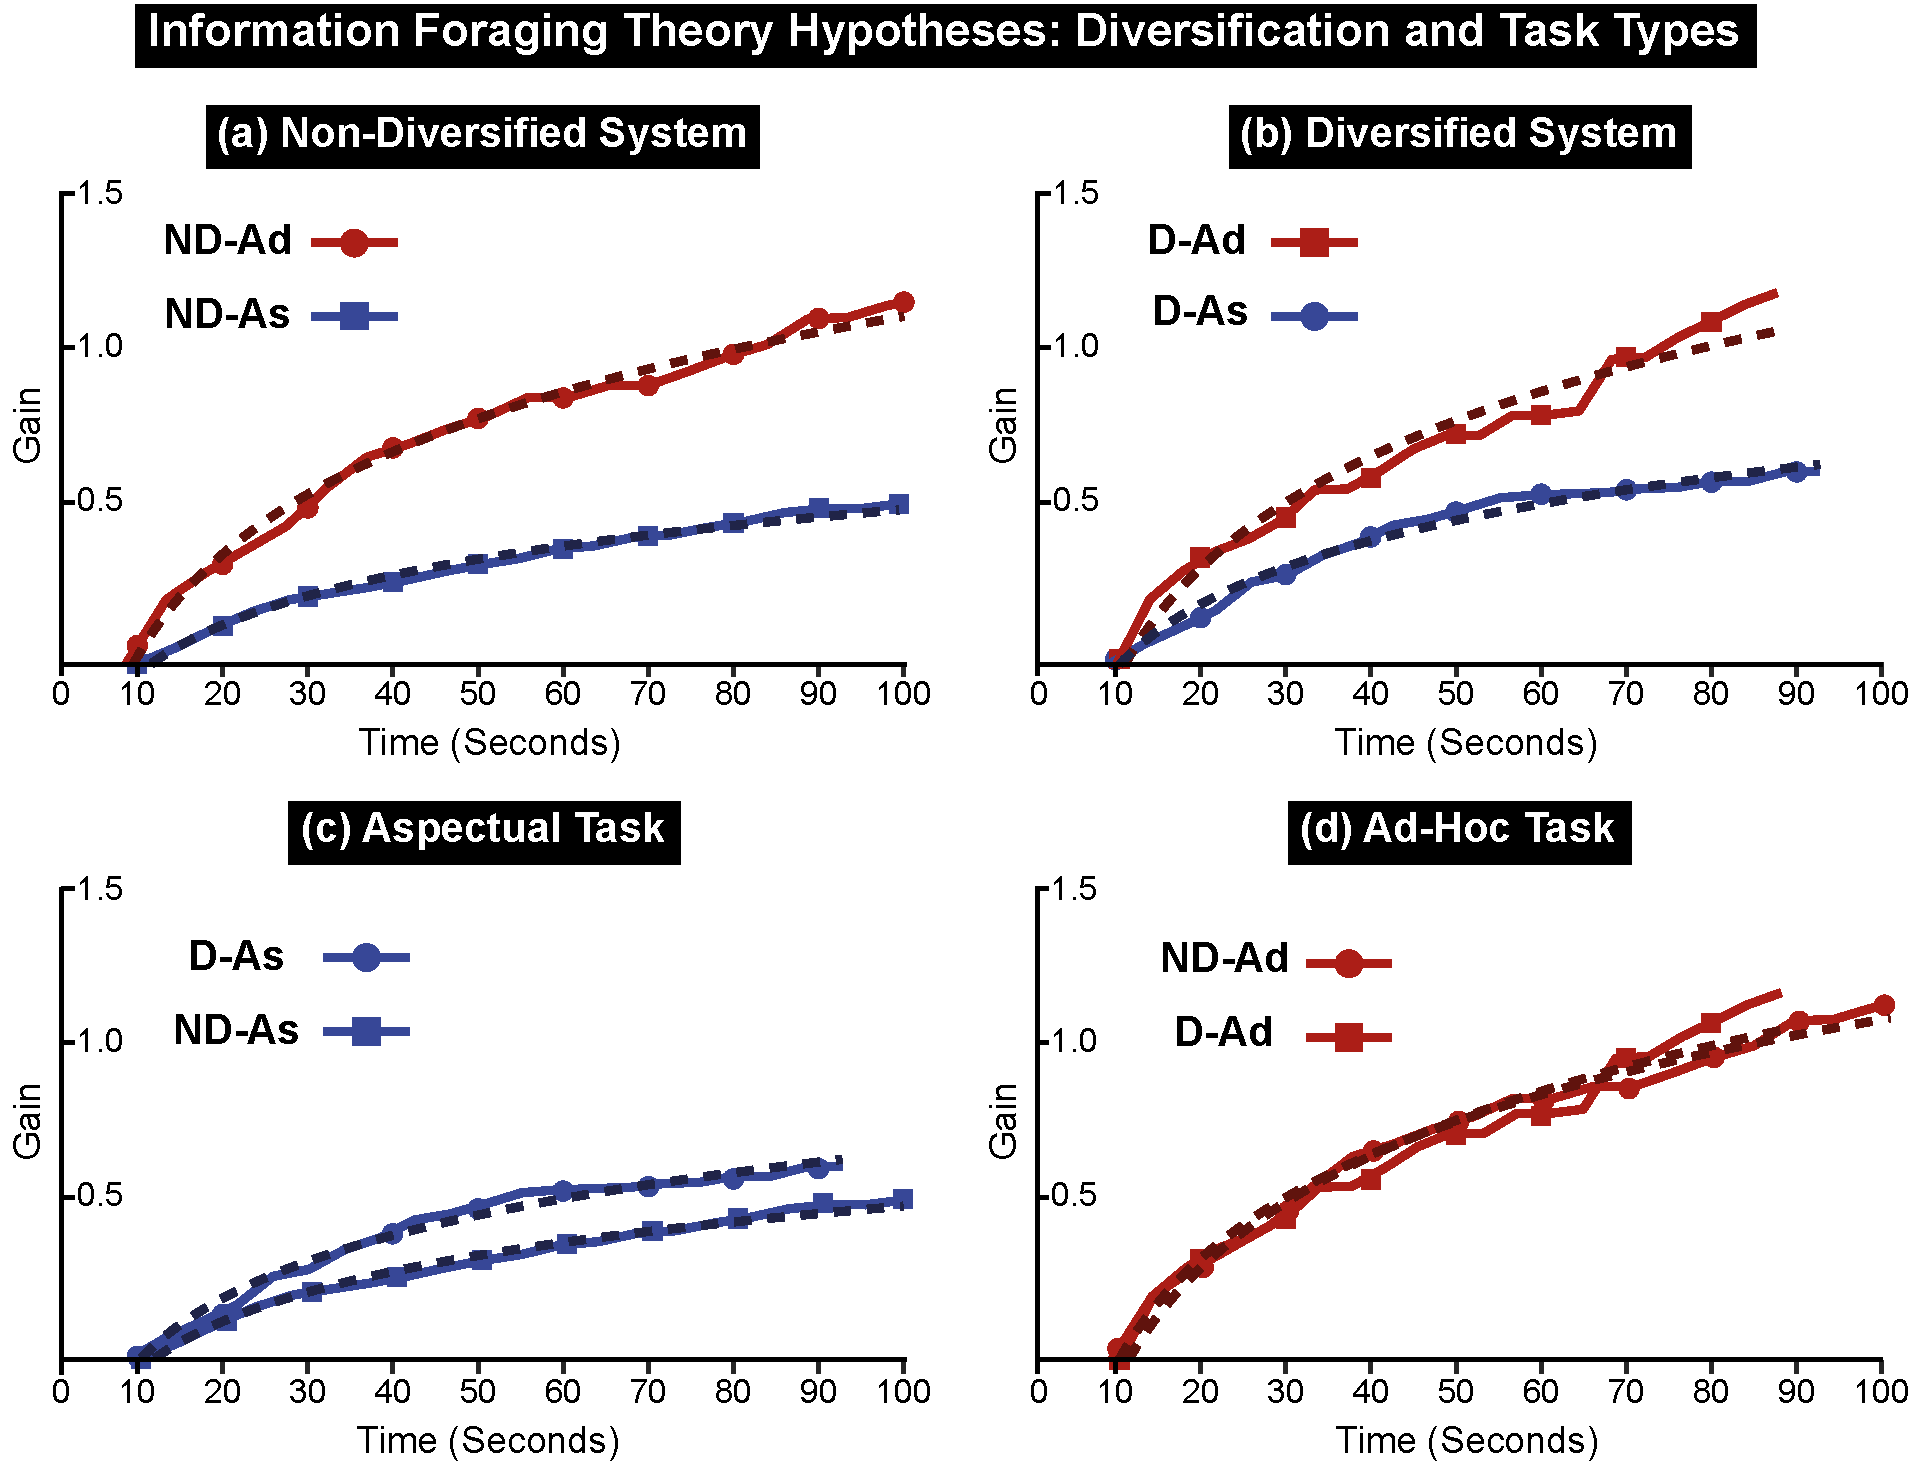
\includegraphics[width=\textwidth]{figures/cg-fromthesis.pdf}
\caption{Plots illustrating the \emph{Cumulative Gain (CG)} attained by subjects of the study, on average, over the first 100 seconds of a search session. Plots are analogous to those in Fig.~\ref{fig_ift_patches}. Also included in are fitted curves (dashed lines).} \label{fig_cg}
\end{figure}

%%%%%%%%%%%%%%%
\subsection{Gain over Time}
%%%%%%%%%%%%%%%
We motivated this study using IFT where we constructed a number of gain curves that reflected our beliefs about how the search performance experienced by users would look like over each system and task. This was done to generate the hypotheses mentioned in Section~\ref{sec:questions}. Here, we examine how participants performed over time for each of the systems and conditions to infer the gain curves. We then compare that to our expectations (which were shown previously in Fig.~\ref{fig_ift_patches}).

To create empirical gain curves, we plotted \emph{Cumulative Gain (CG)} over time. Here, we defined gain to be the number of saved relevant documents (in the case of ad-hoc retrieval), and gain as the number of saved relevant but different documents (in the case of aspectual retrieval). These definitions are what we said would constitute a useful document in the two separate tasks. As gain is measured in the same units, we can therefore plot the gain for both tasks on the same axes to aid comparability.

Fig.~\ref{fig_cg} shows the corresponding empirical gain curves for: \textit{\textbf{(a)}} the non-diversified system on both tasks, \textit{\textbf{(b)}} the diversified System on both tasks, \textit{\textbf{(c)}} the aspectual task for both systems, and \textit{\textbf{(d)}} the ad-hoc task for both systems. Compared to our expectations in Fig.~\ref{fig_ift_patches}, on visual inspection, we see that our predictions were roughly in line with the gain experienced. For example, in Fig.~\ref{fig_ift_patches} \textit{\textbf{(a)}}, we hypothesised that on the non-diversified system, participants would experience greater levels of gain, and the empirical gain curves reported in Fig.~\ref{fig_cg} \emph{\textbf{(a)}} show this. A critical difference though is for Fig.~\ref{fig_ift_patches} \textit{\textbf{(b)}} -- where we hypothesised that the gain curves would be similar on the diversified system (up until a point) before the aspectual gain would drop. From examination of Fig.~\ref{fig_cg} \textit{\textbf{(b)}}, it is clear that participants had a very different experience -- and experienced lower gains earlier in their search sessions -- motivating a revision of our expectations.

To do so, we first fit a logarithmic function to each of the gain curves given time (as done by Athukorala et al.~\cite{ath2014ift}), such that:
\begin{equation}
gain = b \cdot log(time) - a.
\end{equation}

Table~\ref{tbl_plot_fitting} shows the parameters and correlation coefficients for fit ($r^2$) for each condition. We then could calculate how many documents a participant would examine by drawing the tangent line to the estimated gain functions from the origin. This resulted in the predicted number of documents examined -- which we see are in line with the actual documents examined. With respect to Fig.~\ref{fig_cg} \textit{\textbf{(b)}}, we see that for the diversified system, the theory, given their performance, suggests that participants should examine more documents per query on the aspectual task than when undertaking the ad-hoc task (i.e. 4.98 to 3.36, respectively). We observed that they examined 3.48 and 3.02 documents per query -- which follows the same trend, but not the same magnitude. Thus, we revised our expectations regarding how people would search differently between these tasks. With respect to \textit{\textbf{H1}}, we see that the theory, given their performance, suggests that participants, when undertaking the aspectual task, would examine fewer documents per query when using the diversified system. This is compared to the non-diversified system (4.36 vs 4.92). Again, we see that they examined 3.02 and 3.65 documents per query respectively, again following the same trend -- but not to the same magnitude. This post-hoc analysis has justified some of our initial hypotheses regarding how search behaviour would change under the different conditions -- but it has also led to us revising our expectations based on the observed, empirical data.

%We now turn our attention to examining the levels of gain that subjects experienced as they undertook search tasks in different experimental conditions. The aim here is to ascertain whether the graphical illustrations shown earlier in Figure~\ref{fig_ift_patches} are supported by empirical data from this study.

%As previously stated in Section~\ref{sec:questions}, the complexity of this study means that the notion of \emph{gain} -- that is, what each subject found during their search tasks -- changes depending upon the experimental condition that they partook in. Ad-hoc retrieval tasks rely only upon the notion of relevance, meaning that in the context of this study, correctly identifying and saving a TREC relevant document would lead to an increase in gain. Conversely, under the aspectual retrieval tasks, the notion here was to find relevant documents, containing at least one new aspect/entity related to the topic. As such, gain for these tasks was measured according to the number of new entities (in the context of a search session), encountered through each saved document. Using these measurements, we were then able to parse the interaction log to determine the levels of \emph{Cumulative Gain (CG)} that subjects attained, on average, over each of the different conditions trialled. The two plots in Figure~\ref{fig_cg} illustrate the levels of CG attained -- the plot on the left concerns ad-hoc retrieval tasks (conditions \textbf{\emph{D.Ad}} and \textbf{\emph{ND.Ad}}), while the plot on the right considers aspectual retrieval (conditions \textbf{\emph{D.As}} and \textbf{\emph{ND.As}}).

%From the data attained, we could also then use IFT to begin to make a series of predictions regarding the number of documents that subjects would examine and their corresponding stopping depths. Table~\ref{tbl_plot_fitting} shows the fitting parameters, with the plots in Figure~\ref{fig_cg} also including dash lines, representing the fitted curve to each data series.


\begin{table}[t]
    \caption{Fitting parameters for the gain curves illustrated in Fig.~\ref{fig_cg} over each experimental condition. Also included are the estimations from the model for the time to examine a document, and the depth to which subjects should go \emph{(Pred. Docs.)} -- as well as the observed number of documents examined \emph{(Actual Docs.)}, and stopping depth (on average).}
    \label{tbl_plot_fitting}
    \renewcommand{\arraystretch}{1.4}
    \begin{center}
    \begin{small}
    \begin{tabulary}{\textwidth}{L{4.2cm}||D{1cm}|D{1cm}|D{1cm}|D{1cm}|D{1cm}}
    %\begin{tabulary}{\textwidth}{c||c|c|c|c|c}
    
    \hline
    
    % OUTPUT FROM script

& \multicolumn{3}{c|}{\textbf{Model Fitting}} & \textbf{Pred.} & \textbf{Actual} \\

\textbf{Experimental Condition} & \boldmath{$a$} & \boldmath{$b$} & \boldmath{$r^2$} &  \hspace*{-0.5mm}\textbf{Docs.} & \hspace*{-0.5mm}\textbf{Docs.}\\ \hline\hline

\textbf{\emph{ND.Ad}} & $-1.08$ & $0.48$ & $0.989$ & $3.68$ & $3.23$  \\ \hline
\textbf{\emph{ND.As}} & $-0.57$ & $0.23$ & $0.987$ & $4.92$ & $3.65$  \\ \hline\hline
\textbf{\emph{D.Ad}} & $-1.22$ & $0.52$ & $0.959$ & $4.98$ & $3.48$  \\ \hline
\textbf{\emph{D.As}} & $-0.68$ & $0.29$ & $0.985$ & $4.36$ & $3.02$  \\ \hline
    % END OUTPUT
    \end{tabulary}
    \end{small}
    \end{center}
\end{table}

